\begin{problem}{Laser do Léo}{standard input}{standard output}{2 seconds}{256 megabytes}

Leonardo acaba de comprar um laser e decidiu trollar Alberto, um de seus amigos, ao apontar seu laser para ele. Ambos estão na mesma sala, então para que não fique óbvio quem está com o laser, ele decidiu não apontar diretamente, mas através de um espelho. A sala pode ser considerada como um plano cartesiano 2D infinito, em que Leonardo e Alberto são os pontos com coordenadas $(x_L, y_L)$ e $(x_A, y_A)$, respectivamente, e o espelho, que reflete para ambos os lados, é representado por um segmento de reta unindo os pontos $(x_{E1}, y_{E1})$ e $(x_{E2}, y_{E2})$.

\begin{center}
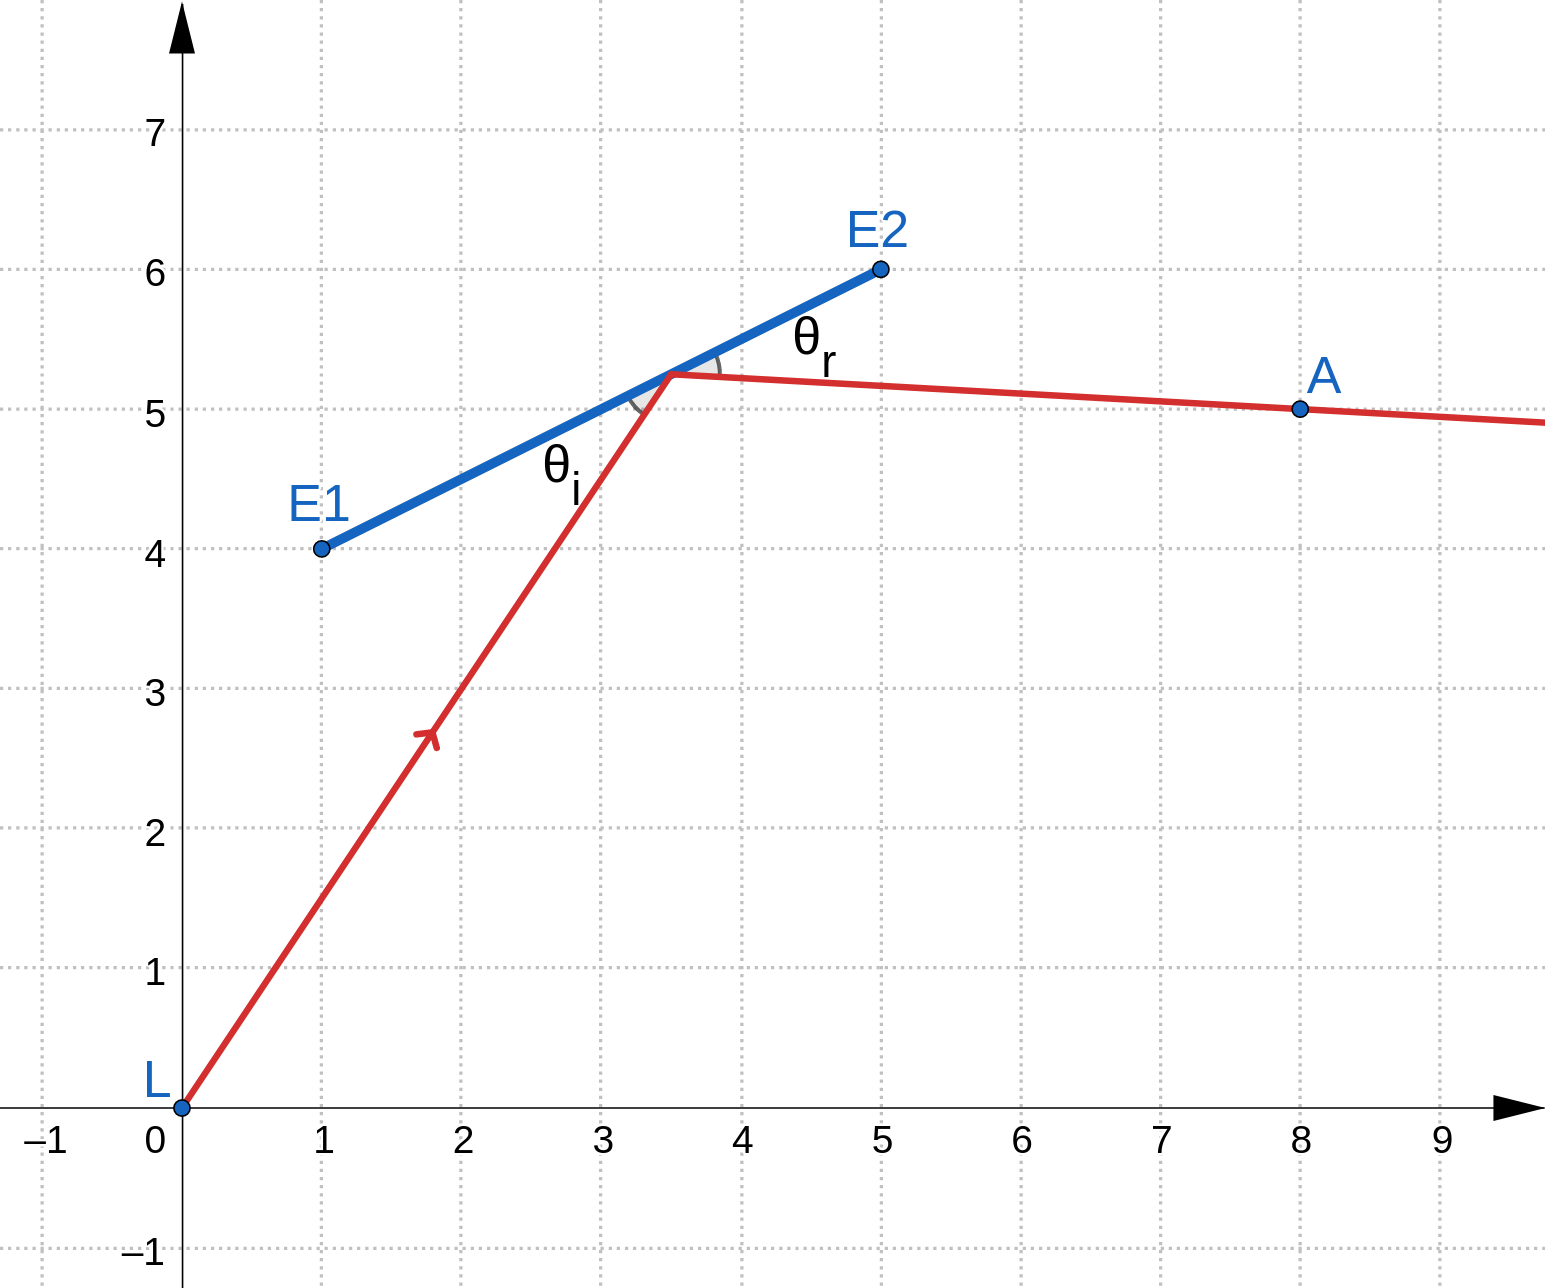
\includegraphics[width=12.0cm, height=9.5cm]{Teste1.png}

Imagem do primeiro caso de teste.
\end{center}

Leonardo é estudioso e sabe que o espelho em questão respeita as leis da física, ou seja, o ângulo de incidência é sempre igual ao ângulo de reflexão ($\theta_i = \theta_r$).

O espelho divide o plano em dois semi-planos. É garantido que Leonardo e Alberto estão localizados no mesmo semi-plano e que nenhum dos dois está em posição colinear com o espelho, e é possível desconsiderar Alberto e Leonardo como obstáculos, ou seja, o laser simplesmente os atravessa.

Ajude Leonardo a saber se é possível atingir Alberto com o laser através do espelho.

\InputFile
A primeira linha da entrada contém um inteiro $T$ ($1 \le T \le 10^4$) indicando o número de casos de testes.

A primeira linha de cada caso de teste contém quatro inteiros $x_L, y_L, x_A, y_A$ ($-500 \le x_L, y_L, x_A, y_A \le 500$), representando as coordenadas de Leonardo e Alberto, respectivamente.

A segunda linha contém outros quatro inteiros $x_{E1}$, $y_{E1}$, $x_{E2}$, $y_{E2}$ ($-500 \le x_{E1}, y_{E1}, x_{E2}, y_{E2} \le 500$), representando as coordenadas dos extremos do espelho.

É garantido que nenhum dos quatro pontos $L$, $A$, $E1$ e $E2$ ocupam a mesma posição no espaço.

\OutputFile
Para cada caso de teste, imprima ``De onde veio isso?'' caso Leonardo consiga acertar Alberto com o laser através do espelho, e ``Leo, eu estou te vendo...'' caso contrário.

\Examples

\begin{example}
\exmpfile{example.01}{example.01.a}%
\exmpfile{example.02}{example.02.a}%
\exmpfile{example.03}{example.03.a}%
\exmpfile{example.04}{example.04.a}%
\end{example}

\Note
No segundo caso de teste, é possível acertar Alberto com o laser, como pode ser visto na imagem abaixo:


\begin{center}
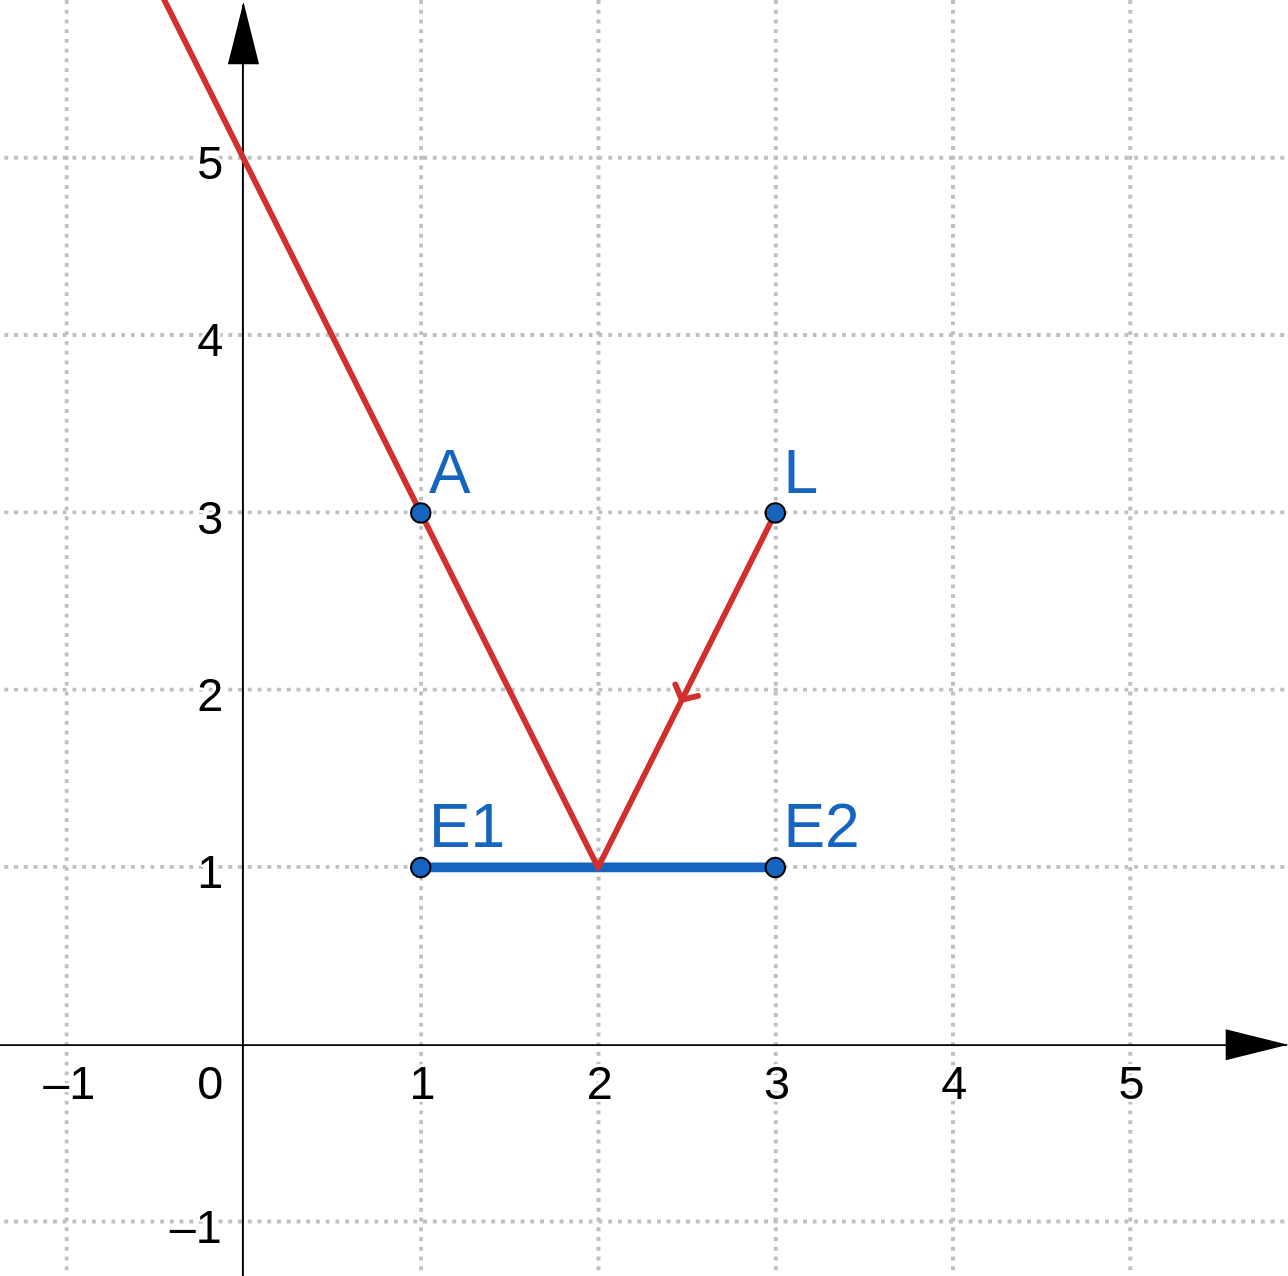
\includegraphics[width=9.5cm, height=9.5cm]{Teste2.png}
\end{center}

No terceiro caso de teste, também é possível acertar Alberto com o laser, pois de acordo com o enunciado, Leonardo e Alberto não são considerados obstáculos pelo laser.

\end{problem}

